\section[Bayesian Inference]{Lecture 2: Bayesian Inference}

'Bayesian Inference' refers to computation of the posterior distribution over parameters given the data.

\begin{itemize}
\item Data $\mathcal{D}=\{t_1, t_2, \ldots, t_N\}$
\item Supervised learning: $\mathcal{D}=\{(x_1,t_1), (x_2,t_2), \ldots, (x_N,t_N)\}$
\item Likelihood function $P(t|w)$ \hspace{1cm}(parameterized by $w$)
\item $P(D|w)= \prod_{n=1}^N P(t_n|w)$ Independence assumption
\item Prior distribution $\pi(w)$
\item Bayes rule: $\mbox{Posterior} \propto \mbox{Likelihood}  \times \mbox{Prior}$
\begin{align}
P(w | D) =\frac{1}{Z} P(D|w) P(w)
\end{align}
\item Probabilities must normalize to $1$: 
\begin{align}
Z= P(D)= \int P(D|w) P(w) dw
\end{align}
Marginalization is the difficult part in Bayesian inference, how we can get arund this step will be shown in a later section
\end{itemize}

\subsection{Usage of the posterior distribution}

	\begin{itemize}
		\item Predictive Distribution
		\begin{align}
			P(t^*|x^*, D)= \int_w P(t^*| x^*, w) P(w| D)   dw
		\end{align}
		where $(t^*,x^*)$ is a new observation

		\item Decision making
		Suppose we have calculated $P(t^*|x^*, D)$, and someone asks us to give a guess $\hat t$ of $t^*$. While we could just take the \emph{most likely value} of $t^*$, it really depends on the cost function. Are mistakes in one direction as costly as mistakes in the other direction? For example, what is the cost of a false positive or false negative? Given a {cost function} $C(\hat t, t)$, one can calculate the 'Bayes-optimal' decision from the posterior distribution. 
		\item Scientific statements
		e.g. 'After observing 100 data points, we were 90\% sure that the parameter $\theta$ is between -.1 and .3. Now that we have observed another 200, we are 97\% sure.'
	\end{itemize}
	
\subsection{Alternatives to a full Bayesian treatment}
In most cases, the posterior distribution can not be calculated exactly, and approximations have to be used.
\begin{itemize}
\item Ignore prior, maximize likelihood $P(D|w)$: {Maximum likelihood learning}
\item Only search for mode of posterior ({Maximum a posteriori, MAP}), i.e. $\mbox{argmax}_w P(w |D) $. In practice, maximize log-posterior.\\
\end{itemize}

\begin{bbbox}{Maximum a posteriori}
\textcolor{gray}{Q: Why is finding the mode of the posterior so much easier than finding the full posterior?}\\
It is a point estimate similar to ML, this makes the approach similarly expensive in computational terms.
We can escape the intractability of the normalization constant.

\textcolor{gray}{Q: When is MAP a really bad idea?}
\begin{itemize}
	\item multiple local maxima
	\item Very skewed posterior distribution
\end{itemize} 
\end{bbbox}

\begin{itemize}
\item Use simplified model to approximate posterior: Find parameters of model $q(w,\Phi)$ such that
$q(w) \approx P(w|D)$. \\

\item Examples: Varational Inference, Expectation Propagation, Laplace Approximation
\item Very often, a Normal approximation is used: $q(w) \approx \mathcal{N}(w|\mu,\Sigma)$.
\item Use MCMC sampling to generate samples from posterior distribution
\end{itemize}

		

\subsection{Coin flip example}
\begin{itemize}
\item Suppose we have $N$ throws of a coin, $D=\{t_1, t_2, \ldots, t_N\}$
\item We write $T_n= 1$ if the n-th throw was head, and $t_n=0$ if it was tail.
\item One parameter:  $q\in [0, 1]$, the probability of obtaining heads
\item Likelihood of one throw:
\begin{align}
 P(T_n=1|q)&= q\\
 P(T_n=0|q)&= (1-q)
\end{align}
Multiple throws: Bernoulli process
\item Likelihood of data $D$: [on board]
\end{itemize}
\begin{bbbox}{Bernoulli likelihood}
\begin{flalign*}
	P(T_n = t | q) &= q^t (1-q)^{1-t}  \\
	P(D | q) &= \prod_{n_1}^N q^{t_n} (1-q)^{1-t_n}
\end{flalign*}
\end{bbbox}

\subsubsection{The beta distribution as a conjugate prior for the Bernoulli distribution}
The shape of the distribution is determined by two parameters.

\begin{figure}
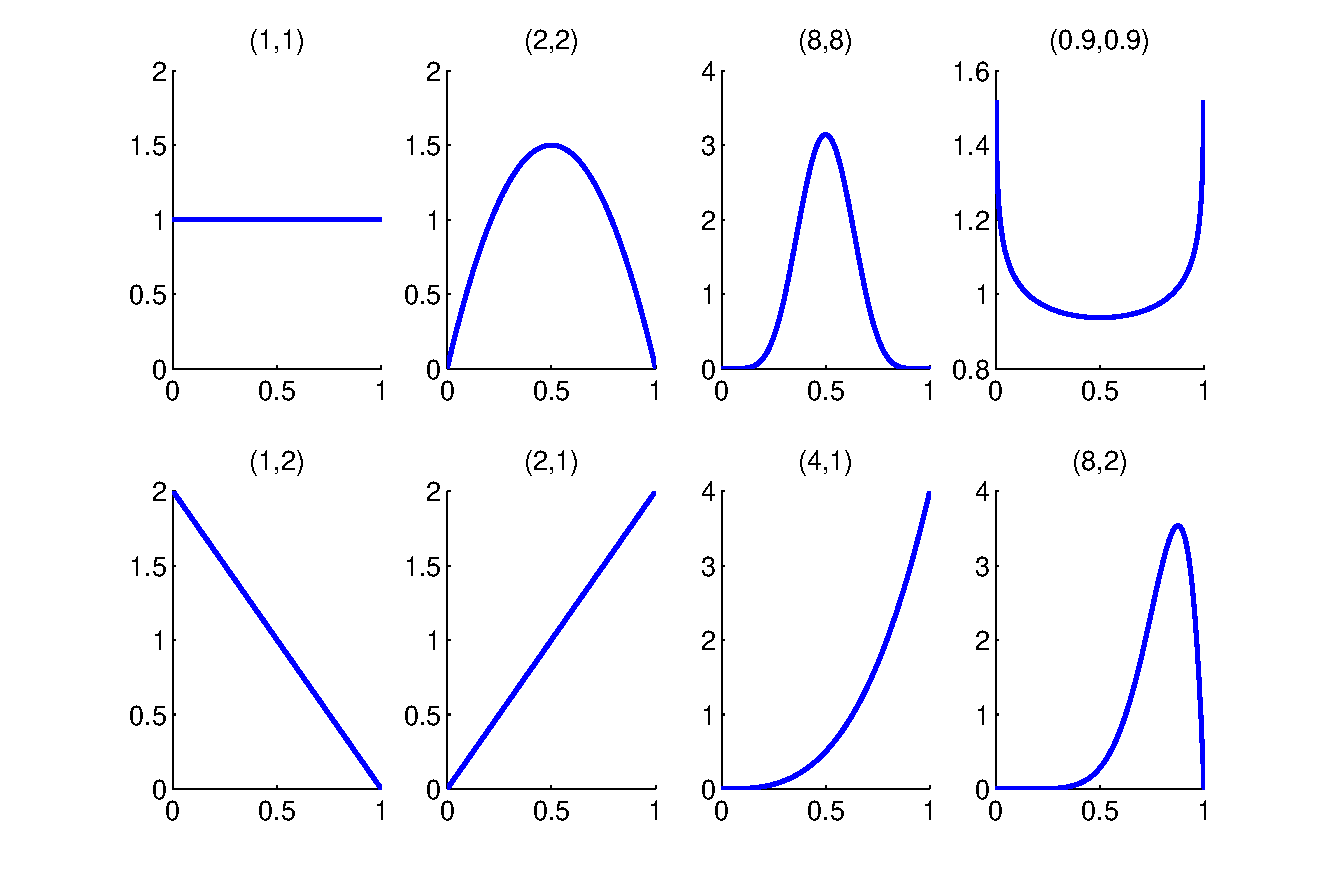
\includegraphics[width=\textwidth]{./lecture2/BetaZoo}
\caption{The beta distribution for different parameter configurations. Notice the symmetricity for $\alpha_1 = \alpha_2$. A prior distribution reflects our beliefs about the parameters. If we have no beliefs we will stick to a flat prior in the upper left corner. Whereas if we believe $q$ to be close to $1$ we might prefer to use the prior in the lower left corner.}
\end{figure}


\begin{itemize}
\item 
Beta distribution: 
\begin{align}
\pi(q| \alpha, \alpha_{2})= \frac{1}{Z}q^{\alpha_1-1} (1-q)^{\alpha_{2}-1}
\end{align}
\item Normalizing constant: the 'beta function'
\begin{align}
Z= \int_0^1 q^{\alpha_1-1} (1-q)^{\alpha_{2}-1} dq=: B(\alpha_1, \alpha_{2})
\end{align}
However there is no need to calculate this constant due to the conjugacy. We will see more on that in a later section.
\item Mean and Variance:
\begin{align}
\mbox{E}(q|\alpha_1,\alpha_{2})&= \frac{\alpha_1}{\alpha_1+\alpha_{2}}\\
\mbox{Var}(q|\alpha_1,\alpha_{2})&= \frac{\alpha_1\alpha_{2}}{(\alpha_1+\alpha_{2})^2(\alpha_1+\alpha_{2}+1)}
\end{align}
\item Symmetric case and heuristics:  [on board]
\end{itemize}

\begin{bbbox}{Symmetric case and heuristics}
\begin{align*}
	Say: \; \alpha_1 = \alpha_2 \\
	then \mbox{E}(q|\alpha_1,\alpha_{2})&= \frac{\alpha_1}{\alpha_1+\alpha_{2}}\\
	&= \frac{\alpha_1}{2 \alpha_1} = 0.5\\
	\mbox{Var}(q|\alpha_1,\alpha_{2})&= \frac{\alpha_1^2}{(2\alpha_1)^2(2\alpha_1 + 1)} \\
									 &= \frac{1}{4(2\alpha_1 + 1)}
\end{align*}
That means for $\alpha_1 = \alpha_2 \rightarrow \infty : \mbox{Var}(q|\alpha_1,\alpha_{2}) \rightarrow 0$
\end{bbbox}

\subsubsection{Posterior inference}

\begin{bbbox}{Posterior inference}
We use $S_n$ to denote the number of heads on the first $n$ trials.
$S_N = \sum_{n_1}^N t_n$
\vspace{.5cm}
Maximum likelihood estimation:
$L(D,q) = log P(D,q) = \sum_{n_1}^N t_n log(q) + (1-t_n) log(1-q) = log(q) S_N + log(1-q)(N-S_N)$\\
Find the q for which the log likelihood is maximized, such that
$\frac{\partial L(D,q)}{\partial q} = 0$\\
$\frac{\partial L(D,q)}{\partial q} = \frac{S_N}{q} - \frac{N-S_N}{1-q} = 0$\\
$\frac{q}{S_N} = \frac{1-q}{N-S_N}$ \\
$q = \frac{S_N}{N}$
\vspace{.5cm}
[on board]

\vspace{.5cm}
Posterior distribution:
\begin{align}
P(q | D) &= \frac{1}{Z}P(D|q)P(q) \\
&= \frac{1}{Z} \prod_{n=1}^N q^{t_n} (1-q)^{1-t_n} \frac{1}{B(\alpha_1,\alpha_2)} q^{\alpha_1 -1} (1-q)^{\alpha_2 - 1} \nonumber \\
&= \frac{1}{Z_2} q^{S_N} (1-q)^{N - S_N} q^{\alpha_1 -1} (1-q)^{\alpha_2 - 1} \nonumber \\
&= \frac{1}{Z_2} q^{S_N + \alpha_1 -1} (1-q)^{N - S_N + \alpha_2 - 1} \nonumber \\
where \; Z_2 &= B(S_N + \alpha_1, N - S_n + \alpha_2) \nonumber
\end{align}

$q | D \backsim Beta(S_N + \alpha_1, N - S_n + \alpha_2)$ \\
\vspace{.5cm}
[on board]
\end{bbbox}

\vspace{.5cm}
We can either take all the data and calculate the posterior at once, or do it sequentially as new data comes in:
\vspace{.5cm}
[on board]

Data: $D=\{1     1     0     1     1     1     1     1     0\}$

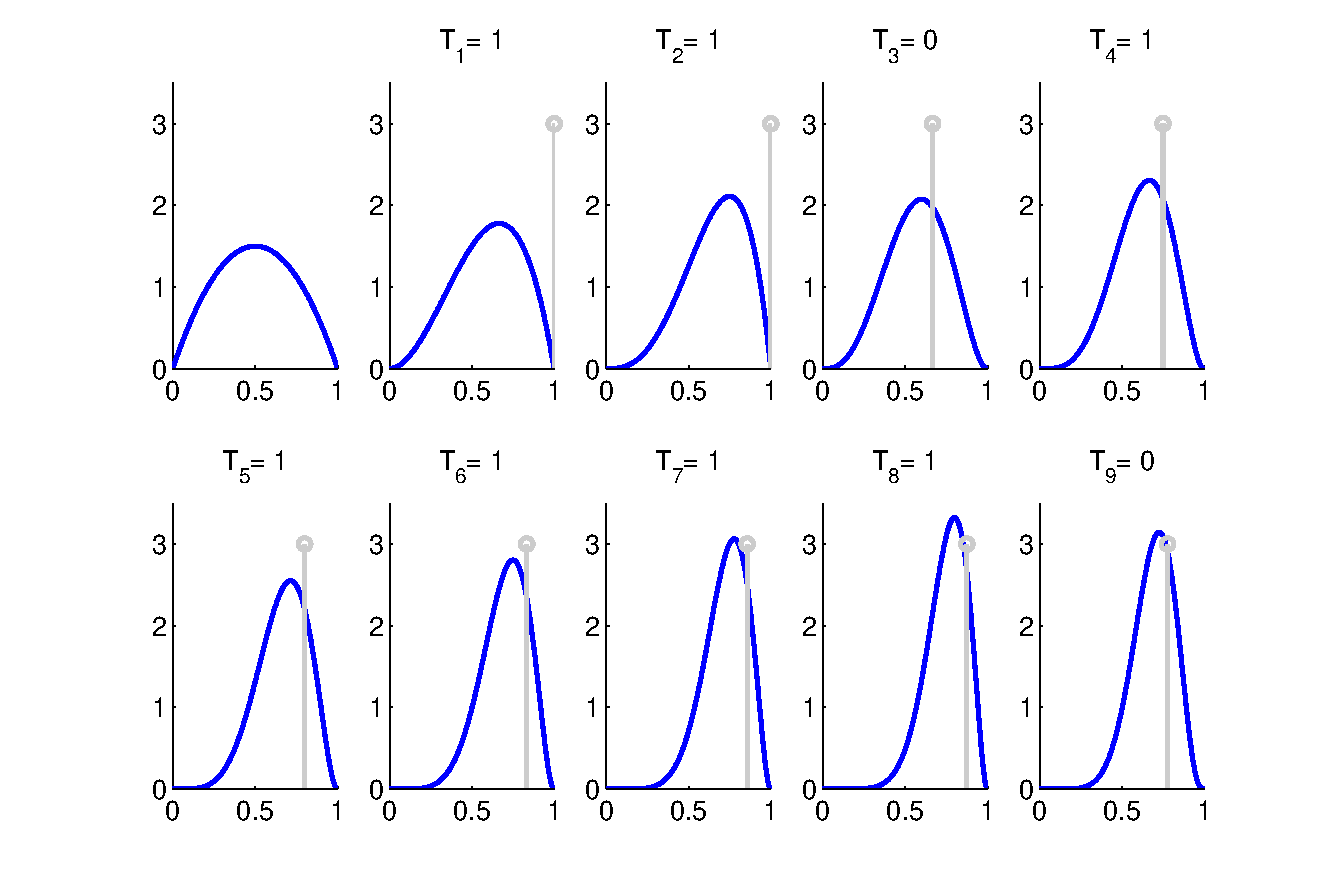
\includegraphics[width=\textwidth]{./lecture2/BetaPosterior}

\subsubsection{Predictive distribution}
\vspace{.5cm}
After observing $N$ coin-flips, what is our prediction for the next coin flip?
\begin{align}
P(T^*=1| D)&= \int_0^1 P(T^*=1|q) P(q|D) dq\\
& = \int_0^1 q P(q|D) dq\\
&= \mbox{E}(q|D) \\
&=\frac{\alpha_1+S_N}{(\alpha_1+ S_N)+(\alpha_{2}+N-S_N)}\\
&=\frac{\alpha_1+S_N}{(\alpha_1+\alpha_2+N)}
\end{align}

\vspace{.5cm}
In our example, $\mbox{E}(q|D)=0.69$, and $\mbox{MLE}=0.78$. 

\begin{bbbox}{What happens if $N$ gets very large?}

For $ \alpha_1,\alpha_2 \rightarrow 0$ or $ S_N , N \rightarrow \infty $ the prediction will approach the maximum likelihood solution.
\end{bbbox}

\vspace{.5cm}
Note: This is a bit of a special case-- in general, the predictive distribution is not simply the likelihood evaluated at the mean!!!


\subsubsection{Statistical Reasoning}
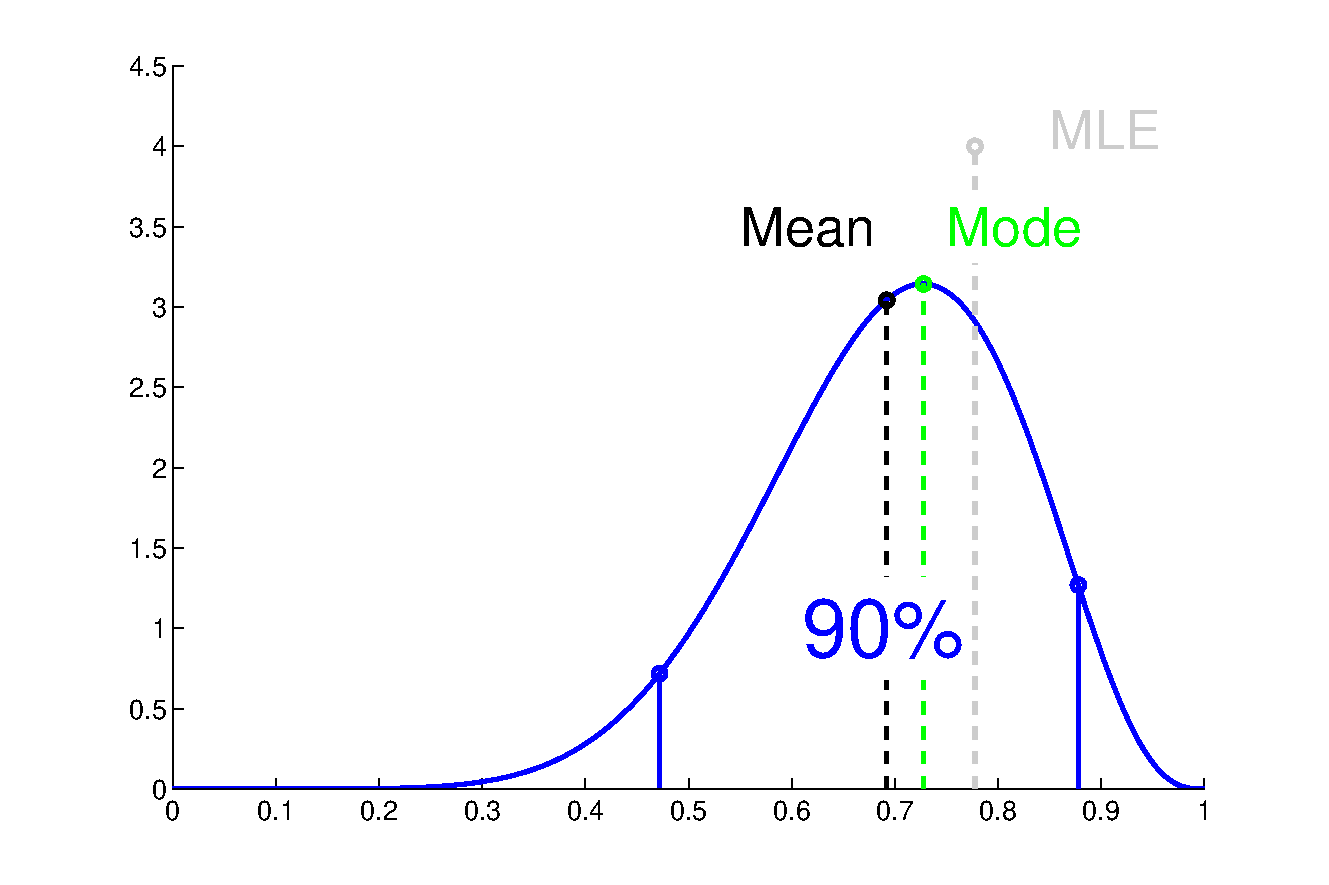
\includegraphics[width=\textwidth]{./lecture2/BetaPosteriorConfidence}

\subsubsection{Decision making}
Someone offers you the bet that you get 1 euros if you predict the next coin toss correctly, but you have to pay 2 euros if if you are wrong. 

Should you take the bet? What should you predict?

\begin{align}
C(t^*,\hat t)=
\begin{cases}
-1 &\mbox{if~} t^*= \hat t\\
2 &\mbox{if~} t^*\neq \hat t\\
\end{cases}
\end{align}

Expected cost: 
\begin{align}
E(C)=\sum_{t^*=0}^1 C(t^*,\hat t) P(t^*| D)
\end{align}

If we predict tail ($t^*=0$): 
\begin{align}
E(C)&= P(t^*=1|D) C(0,1)+P(t^*=0|D) C(0,0)  \\
&=0.69 (2)  + 0.31 (-1)= 1.07
\end{align}

If we predict head ($t^*=1$): 
\begin{align}
E(C)=0.69 (-1)  + 0.31 (2)= -0.07;
\end{align}

\subsection{The exponential family and conjugate priors}
Why was inference so easy here?

\begin{itemize}
\item Posterior distribution had a closed form solution.
\item In fact, the posterior had the same functional form as the prior, just different parameters.
\item Parameters of posterior could be calculated by simply adding observations to prior parameters.
\item We used a likelihood from the {exponential family} and its {conjugate prior}. In this case,  Bayesian inference is always easy.
\item For this reason, exponential families and conjugate priors are used extensively in Bayesian modelling, often as 'building blocks' of more complicated models.
\end{itemize}


Inference is easy whenever the likelihood is in the exponential family and the prior is its conjugate.
\begin{itemize}
\item Exponential family distributions  have the form 
\begin{align}
P(\xx|\theta)&= g(\theta) f(\xx) \exp\left(\phi(\theta)^\top S(\xx)\right)
\end{align}

\item The conjugate prior is
\begin{align}
\pi(\theta)&= F(\tau,\nu) g(\theta)^\nu \exp(\phi(\theta)^\top \tau)
\end{align}
\item Calculating the posterior:
\begin{align}
 [\mbox{on board}]
\end{align}
\end{itemize}

The posterior given an exponential family likelihood and conjugate prior is 
\begin{align}
P(\theta|D)= F(\tau+ \sum_i S(x_i), \nu+N) g(\theta)^{\nu+N} \exp\left(\phi(\theta)^\top(\tau +\sum_i S(x_i)    )\right)
\end{align}

\begin{itemize}
\item $\phi(\theta)$ is the vector of {natural parameters}
\item $\sum_i S(x_i)$ is the vector of {sufficient statistics}
\item $\tau$ are {pseudo-observations}
\item $\nu$ is the scale of the prior\\
\end{itemize}

The exponential family includes most common distributions, including the Normal, Exponential, Gamma, Chi-square, Beta, Dirichlet, Bernoulli, Poisson, Wishart and the Inverse Wishart.

\begin{bbbox}{How can we put our coin-example into this framework?}
\begin{align*}
	P(x | \theta) &= \theta^x (1-\theta)^{1-x} \\
	              &= \theta^x (1-\theta)(1-\theta)^{-x} \\
	              &= (1-\theta) \exp\left(\log\left(\theta^x (1-\theta)^{-x}\right)\right) \\
	              &= (1-\theta) \exp\left(x \log\left(\frac{\theta}{1-\theta}\right)\right) \\
        g(\theta) &= 1 - \theta \\
             f(x) &= 1 \\
     \phi(\theta) &= log\left(\frac{\theta}{1 - \theta}\right) : log odds \\
             S(x) &= x
\end{align*}
\end{bbbox}
